\begin{figure}[H]
    \centering
    \begin{subfigure}[b]{0.49\textwidth}
        \centering
        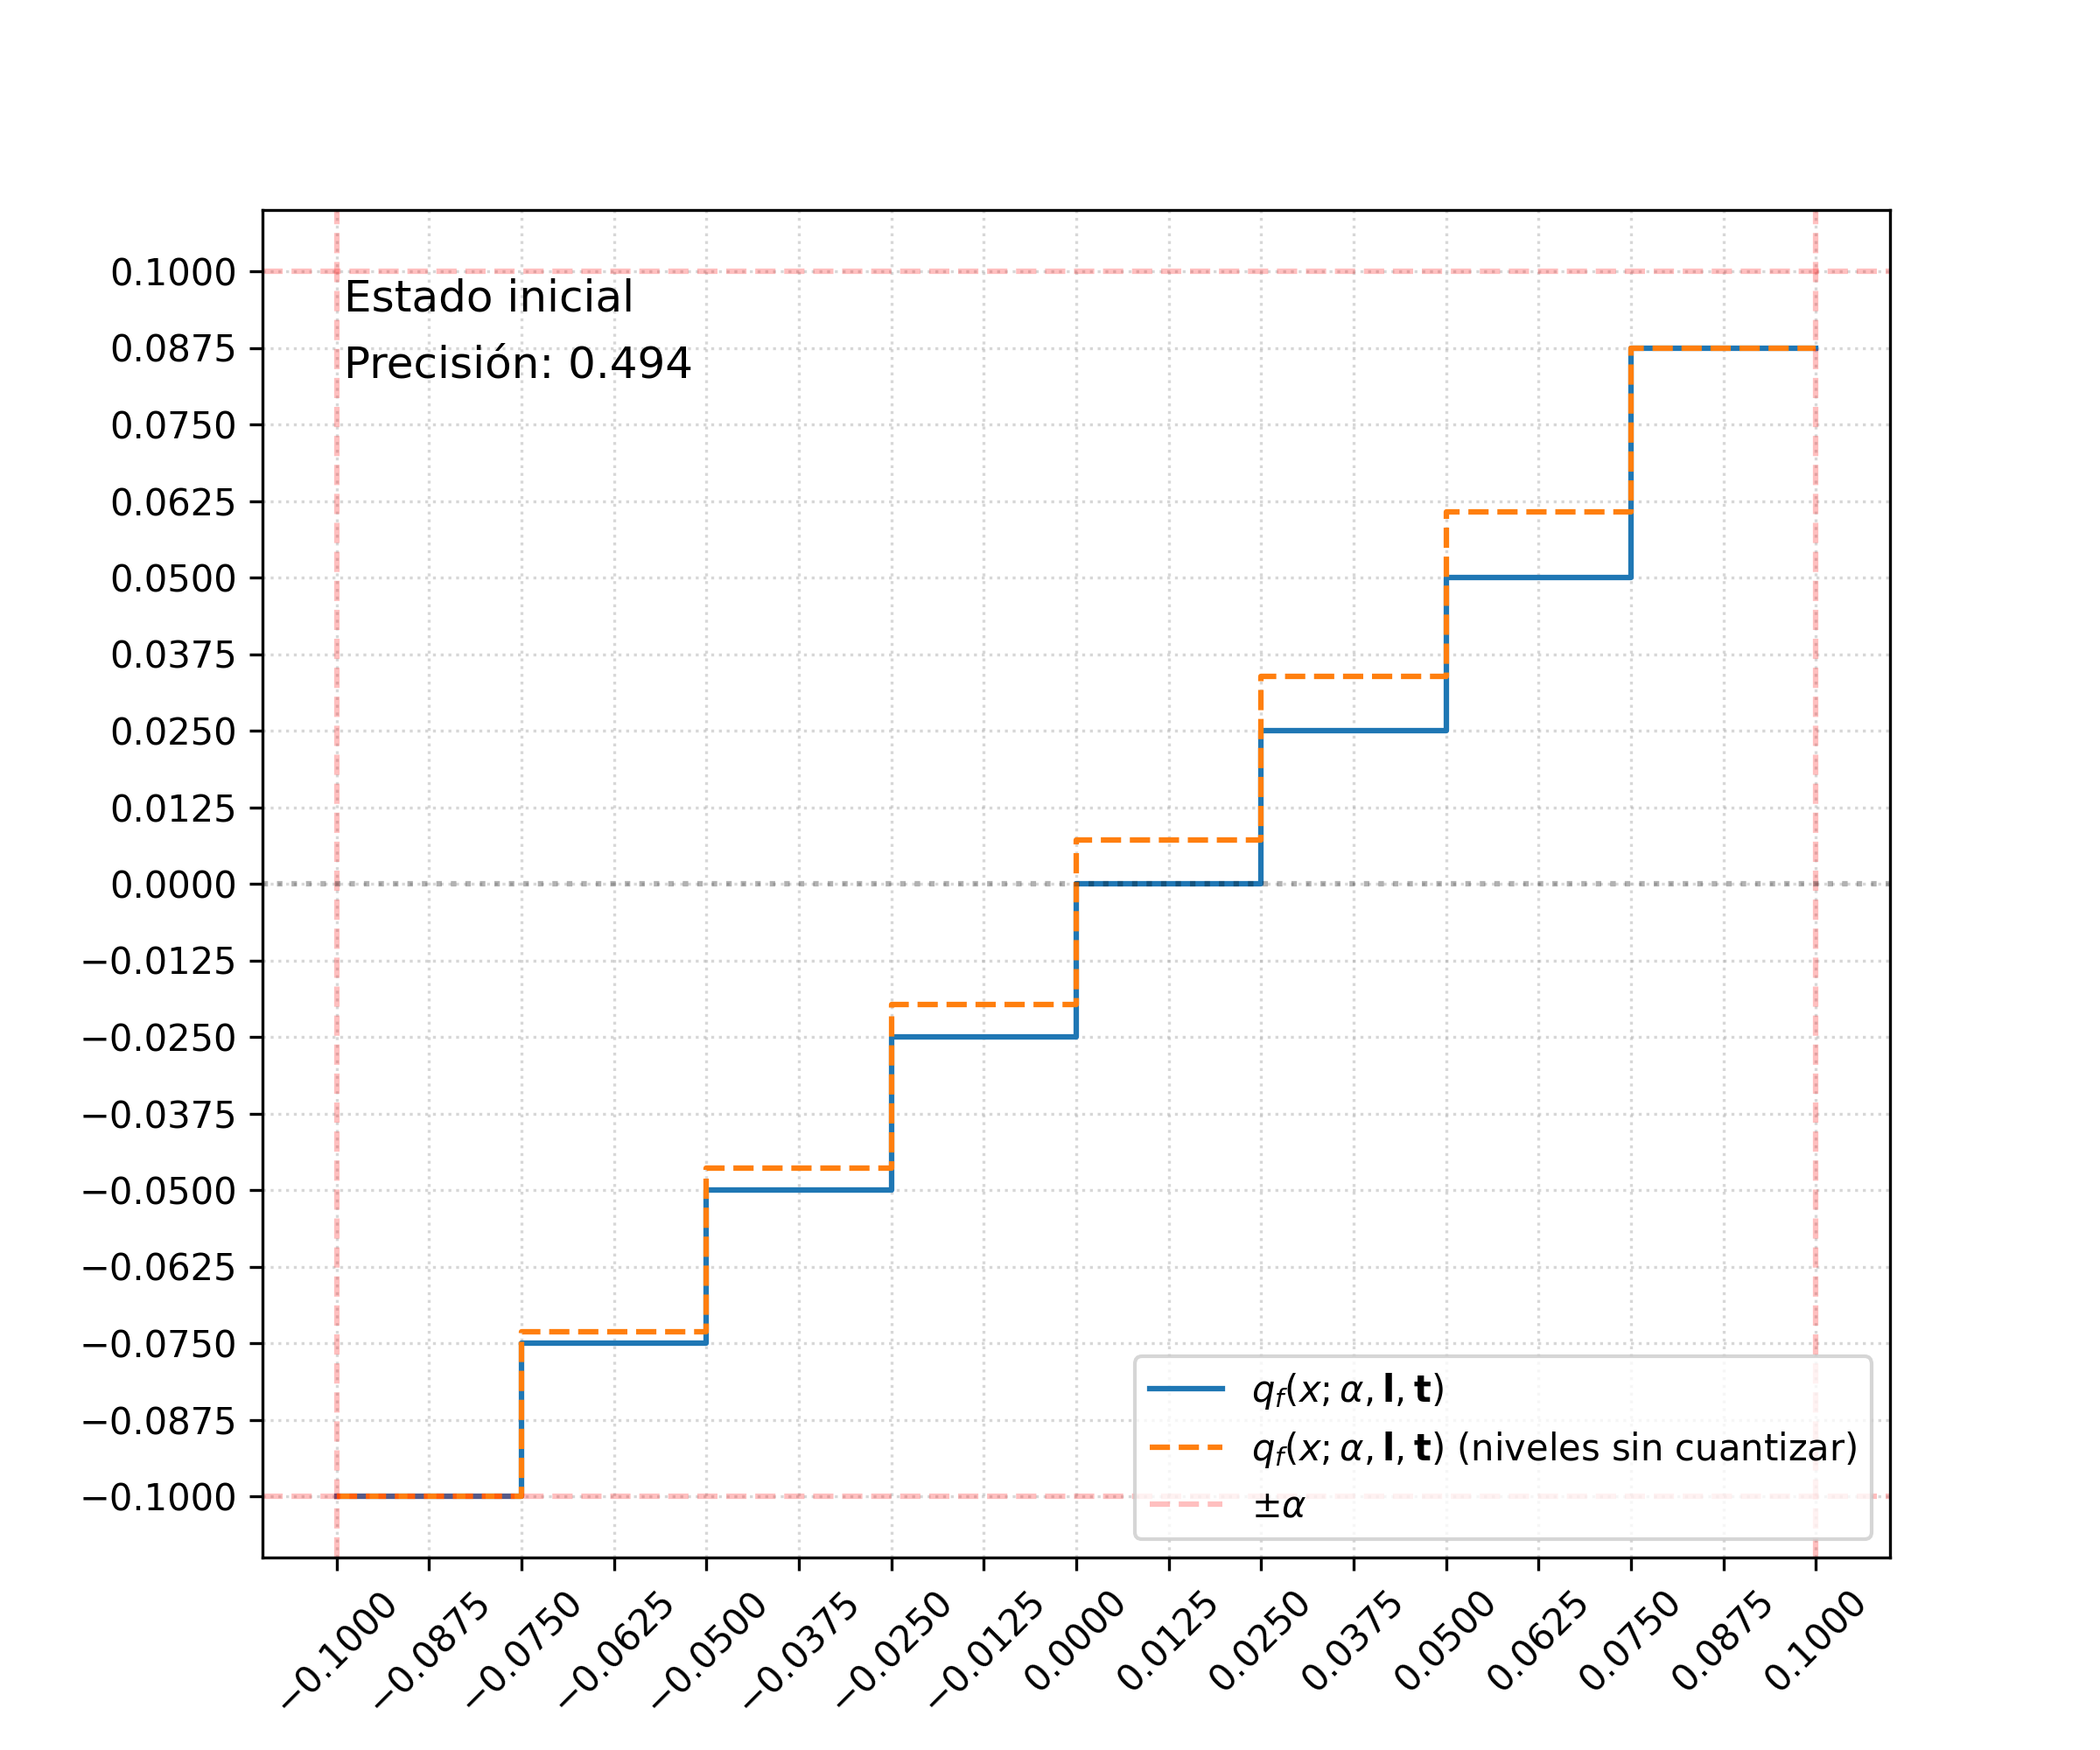
\includegraphics[width=\textwidth]{pics/quantizers/flex_ok/snapshot_00000.png}
        \caption{Estado inicial}
        \label{fig:flexible_snapshot_0}
    \end{subfigure}
    \hfill
    \begin{subfigure}[b]{0.49\textwidth}
        \centering
        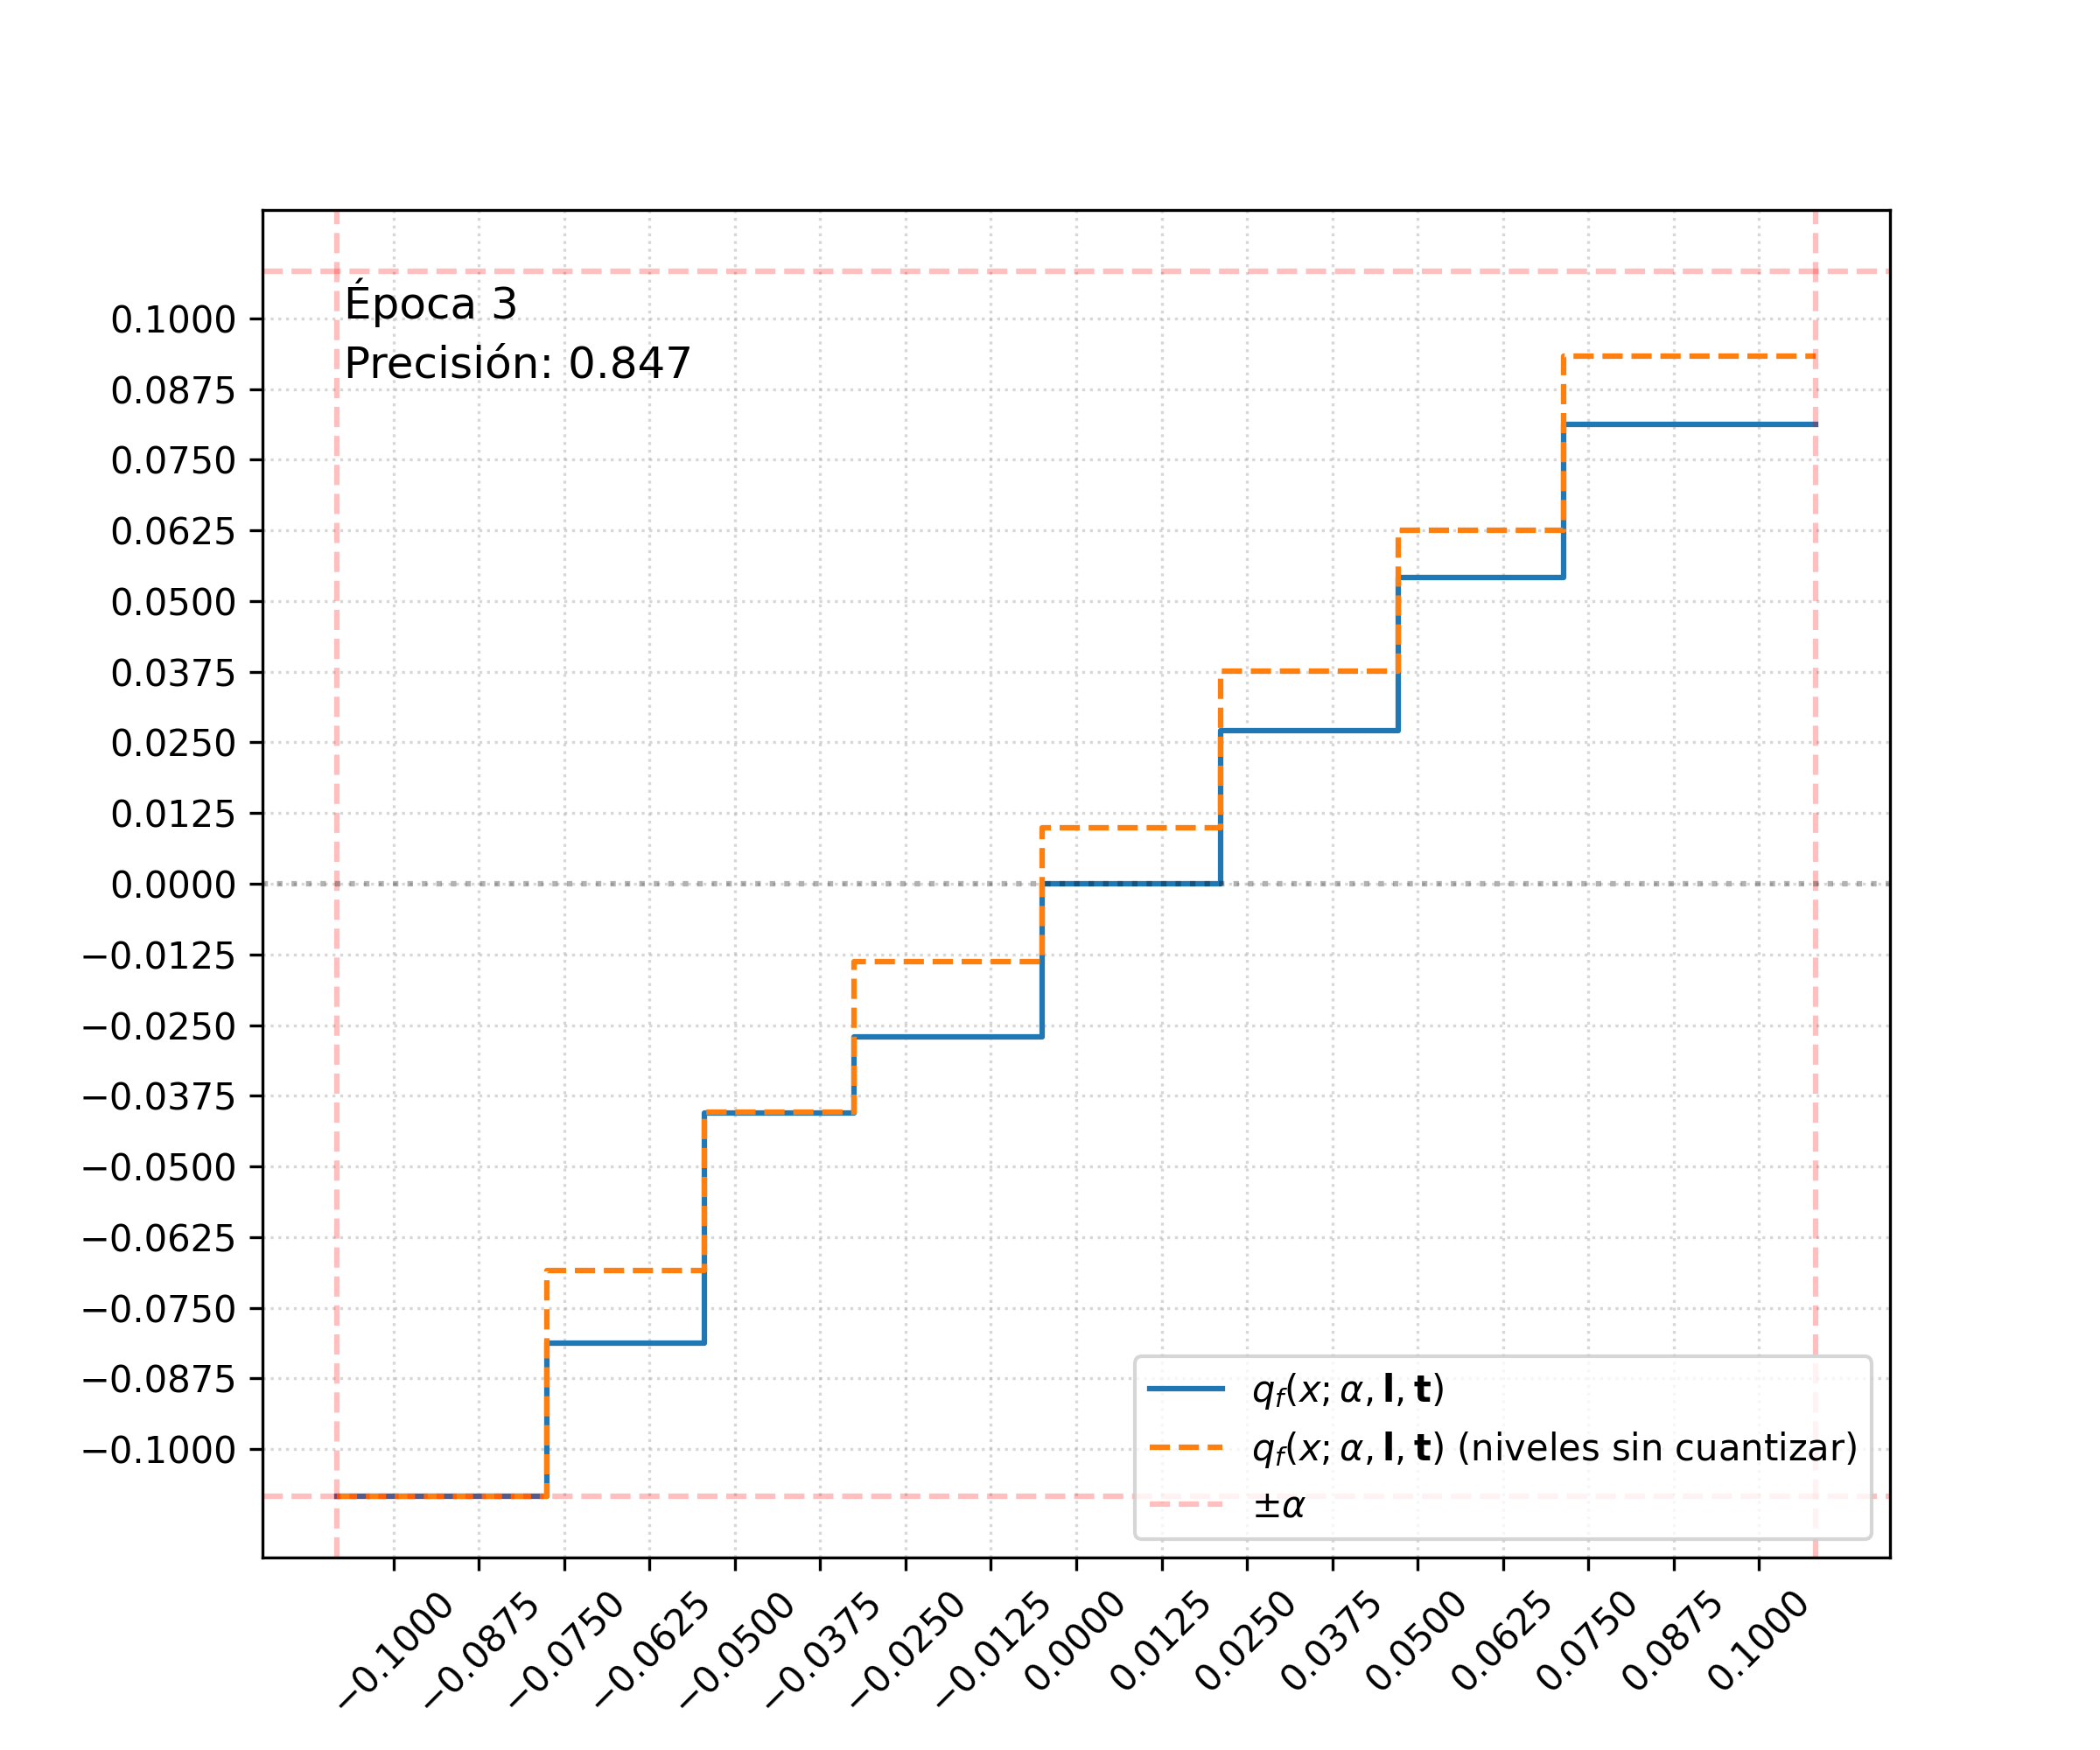
\includegraphics[width=\textwidth]{pics/quantizers/flex_ok/snapshot_00003.png}
        \caption{Época 3}
        \label{fig:flexible_snapshot_3}
    \end{subfigure}

    \vspace{0.5cm}

    \begin{subfigure}[b]{0.49\textwidth}
        \centering
        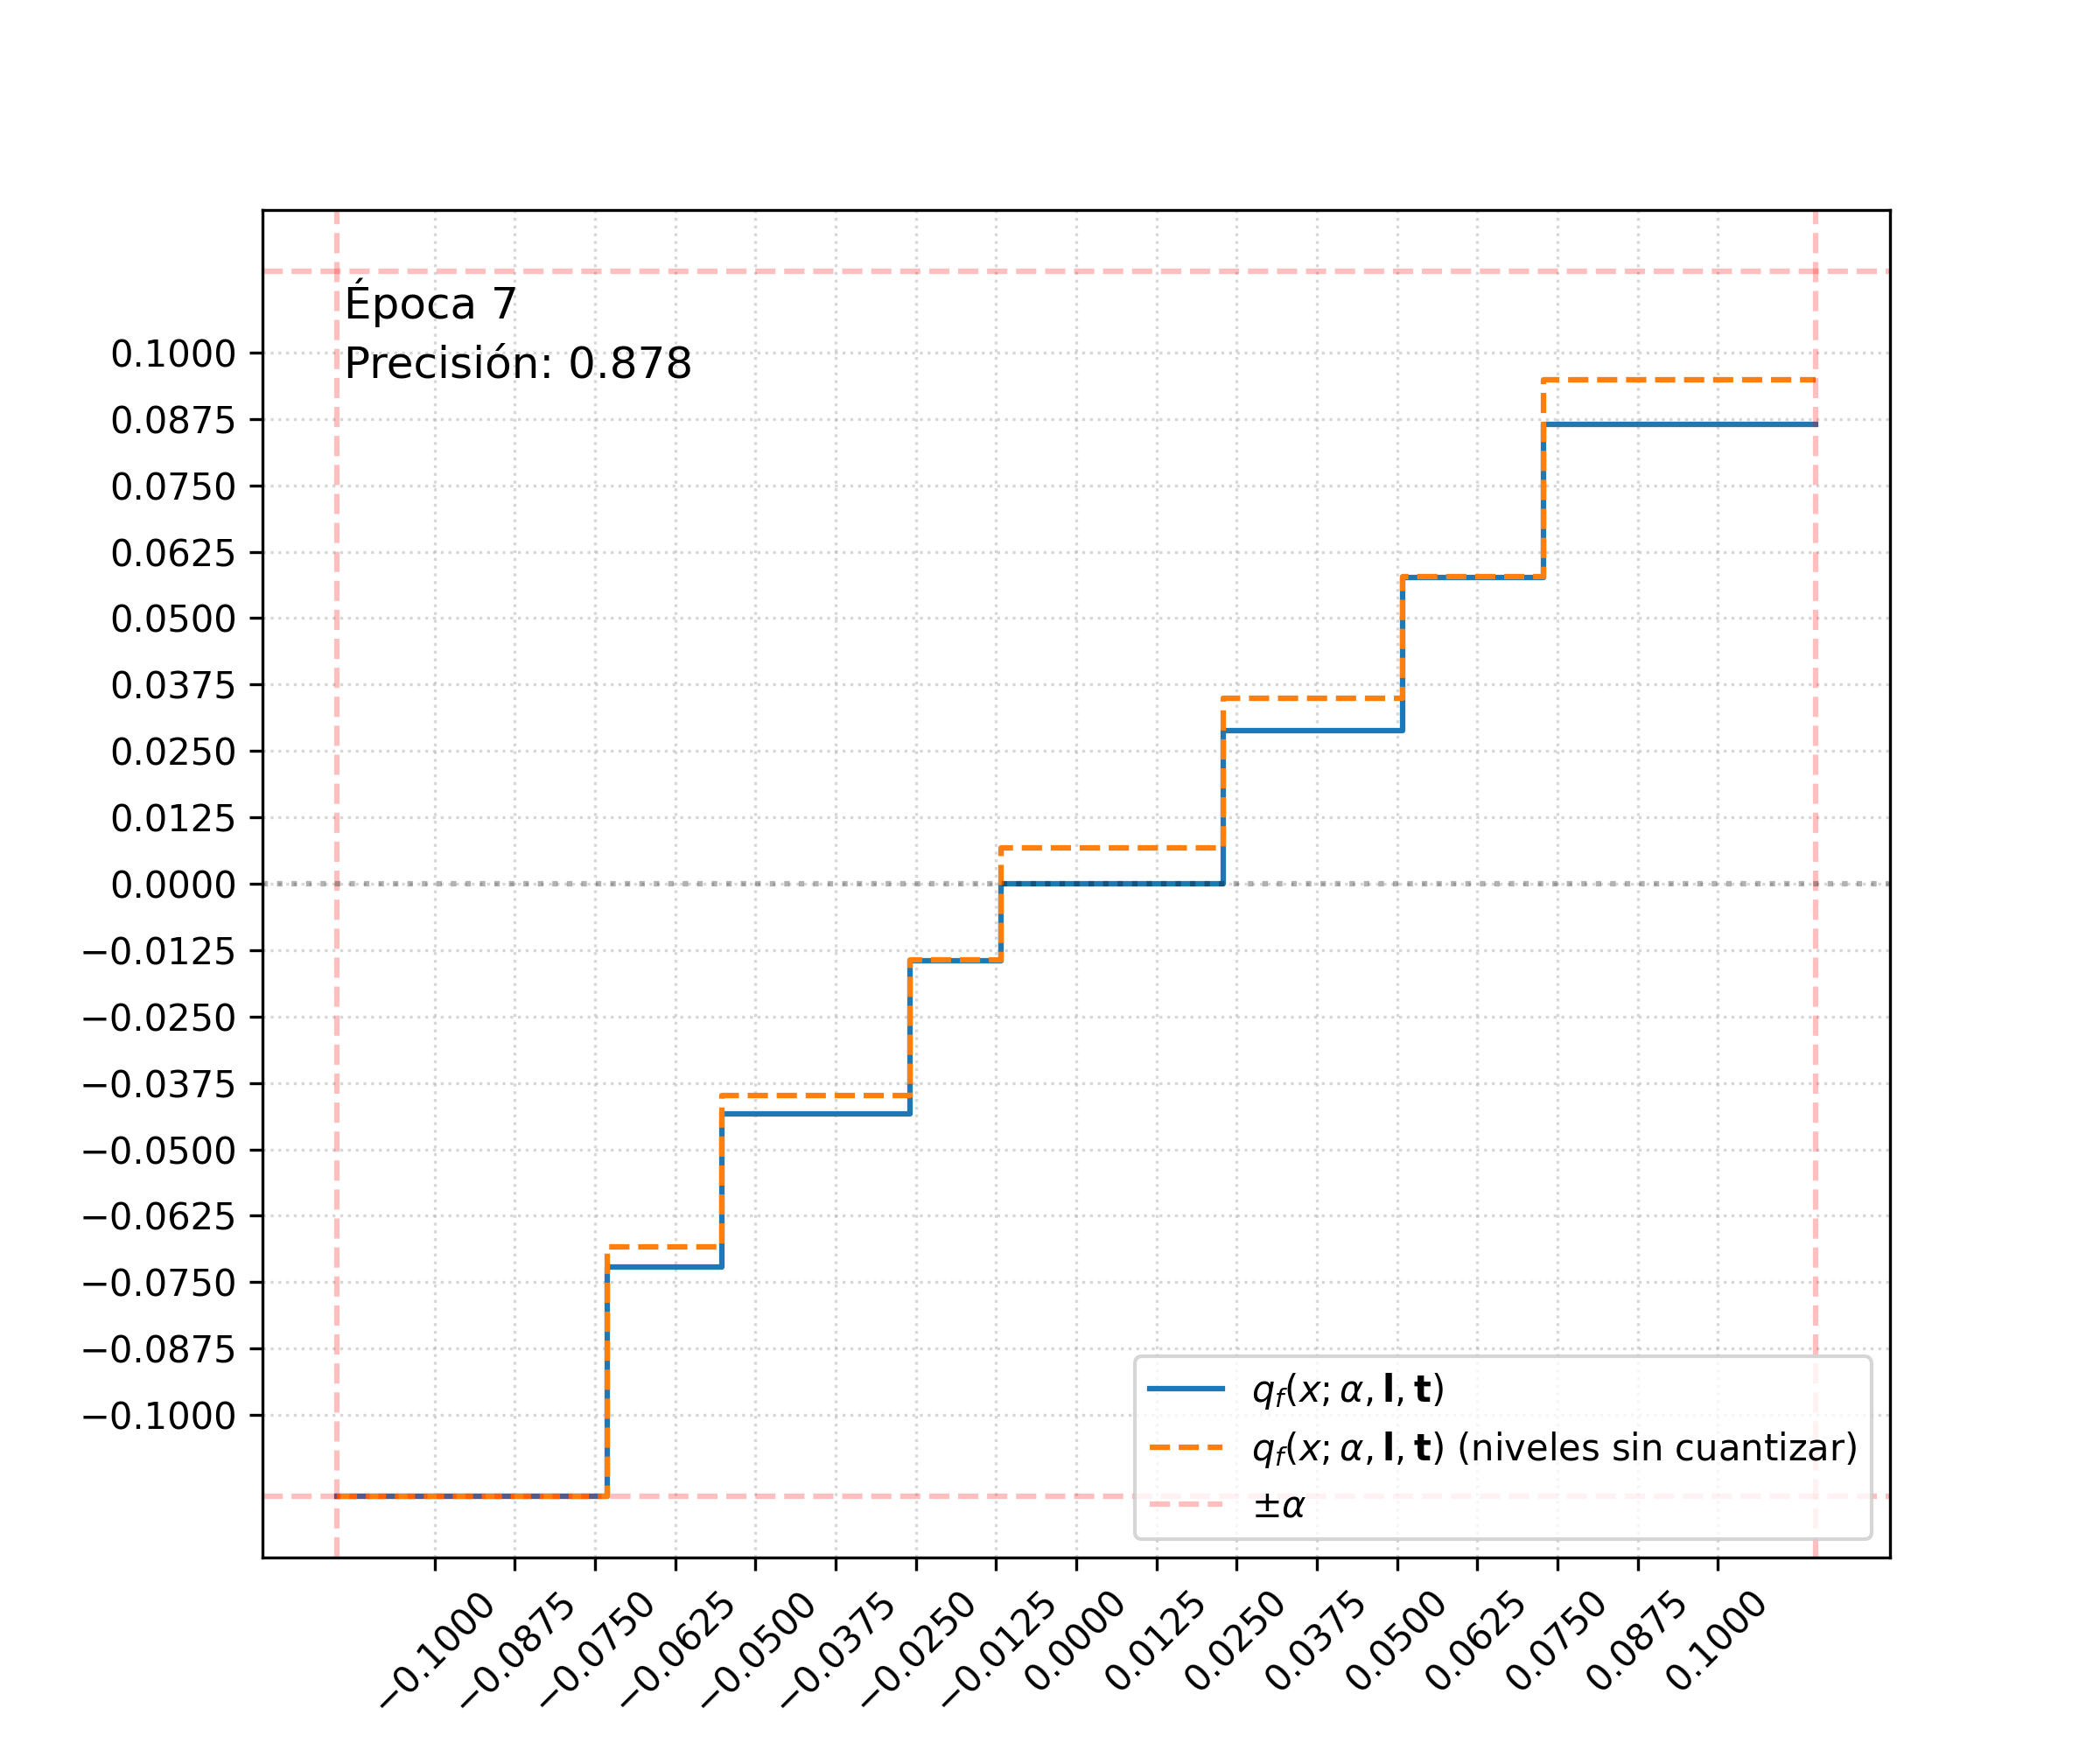
\includegraphics[width=\textwidth]{pics/quantizers/flex_ok/snapshot_00007.png}
        \caption{Época 7}
        \label{fig:flexible_snapshot_7}
    \end{subfigure}
    \hfill
    \begin{subfigure}[b]{0.49\textwidth}
        \centering
        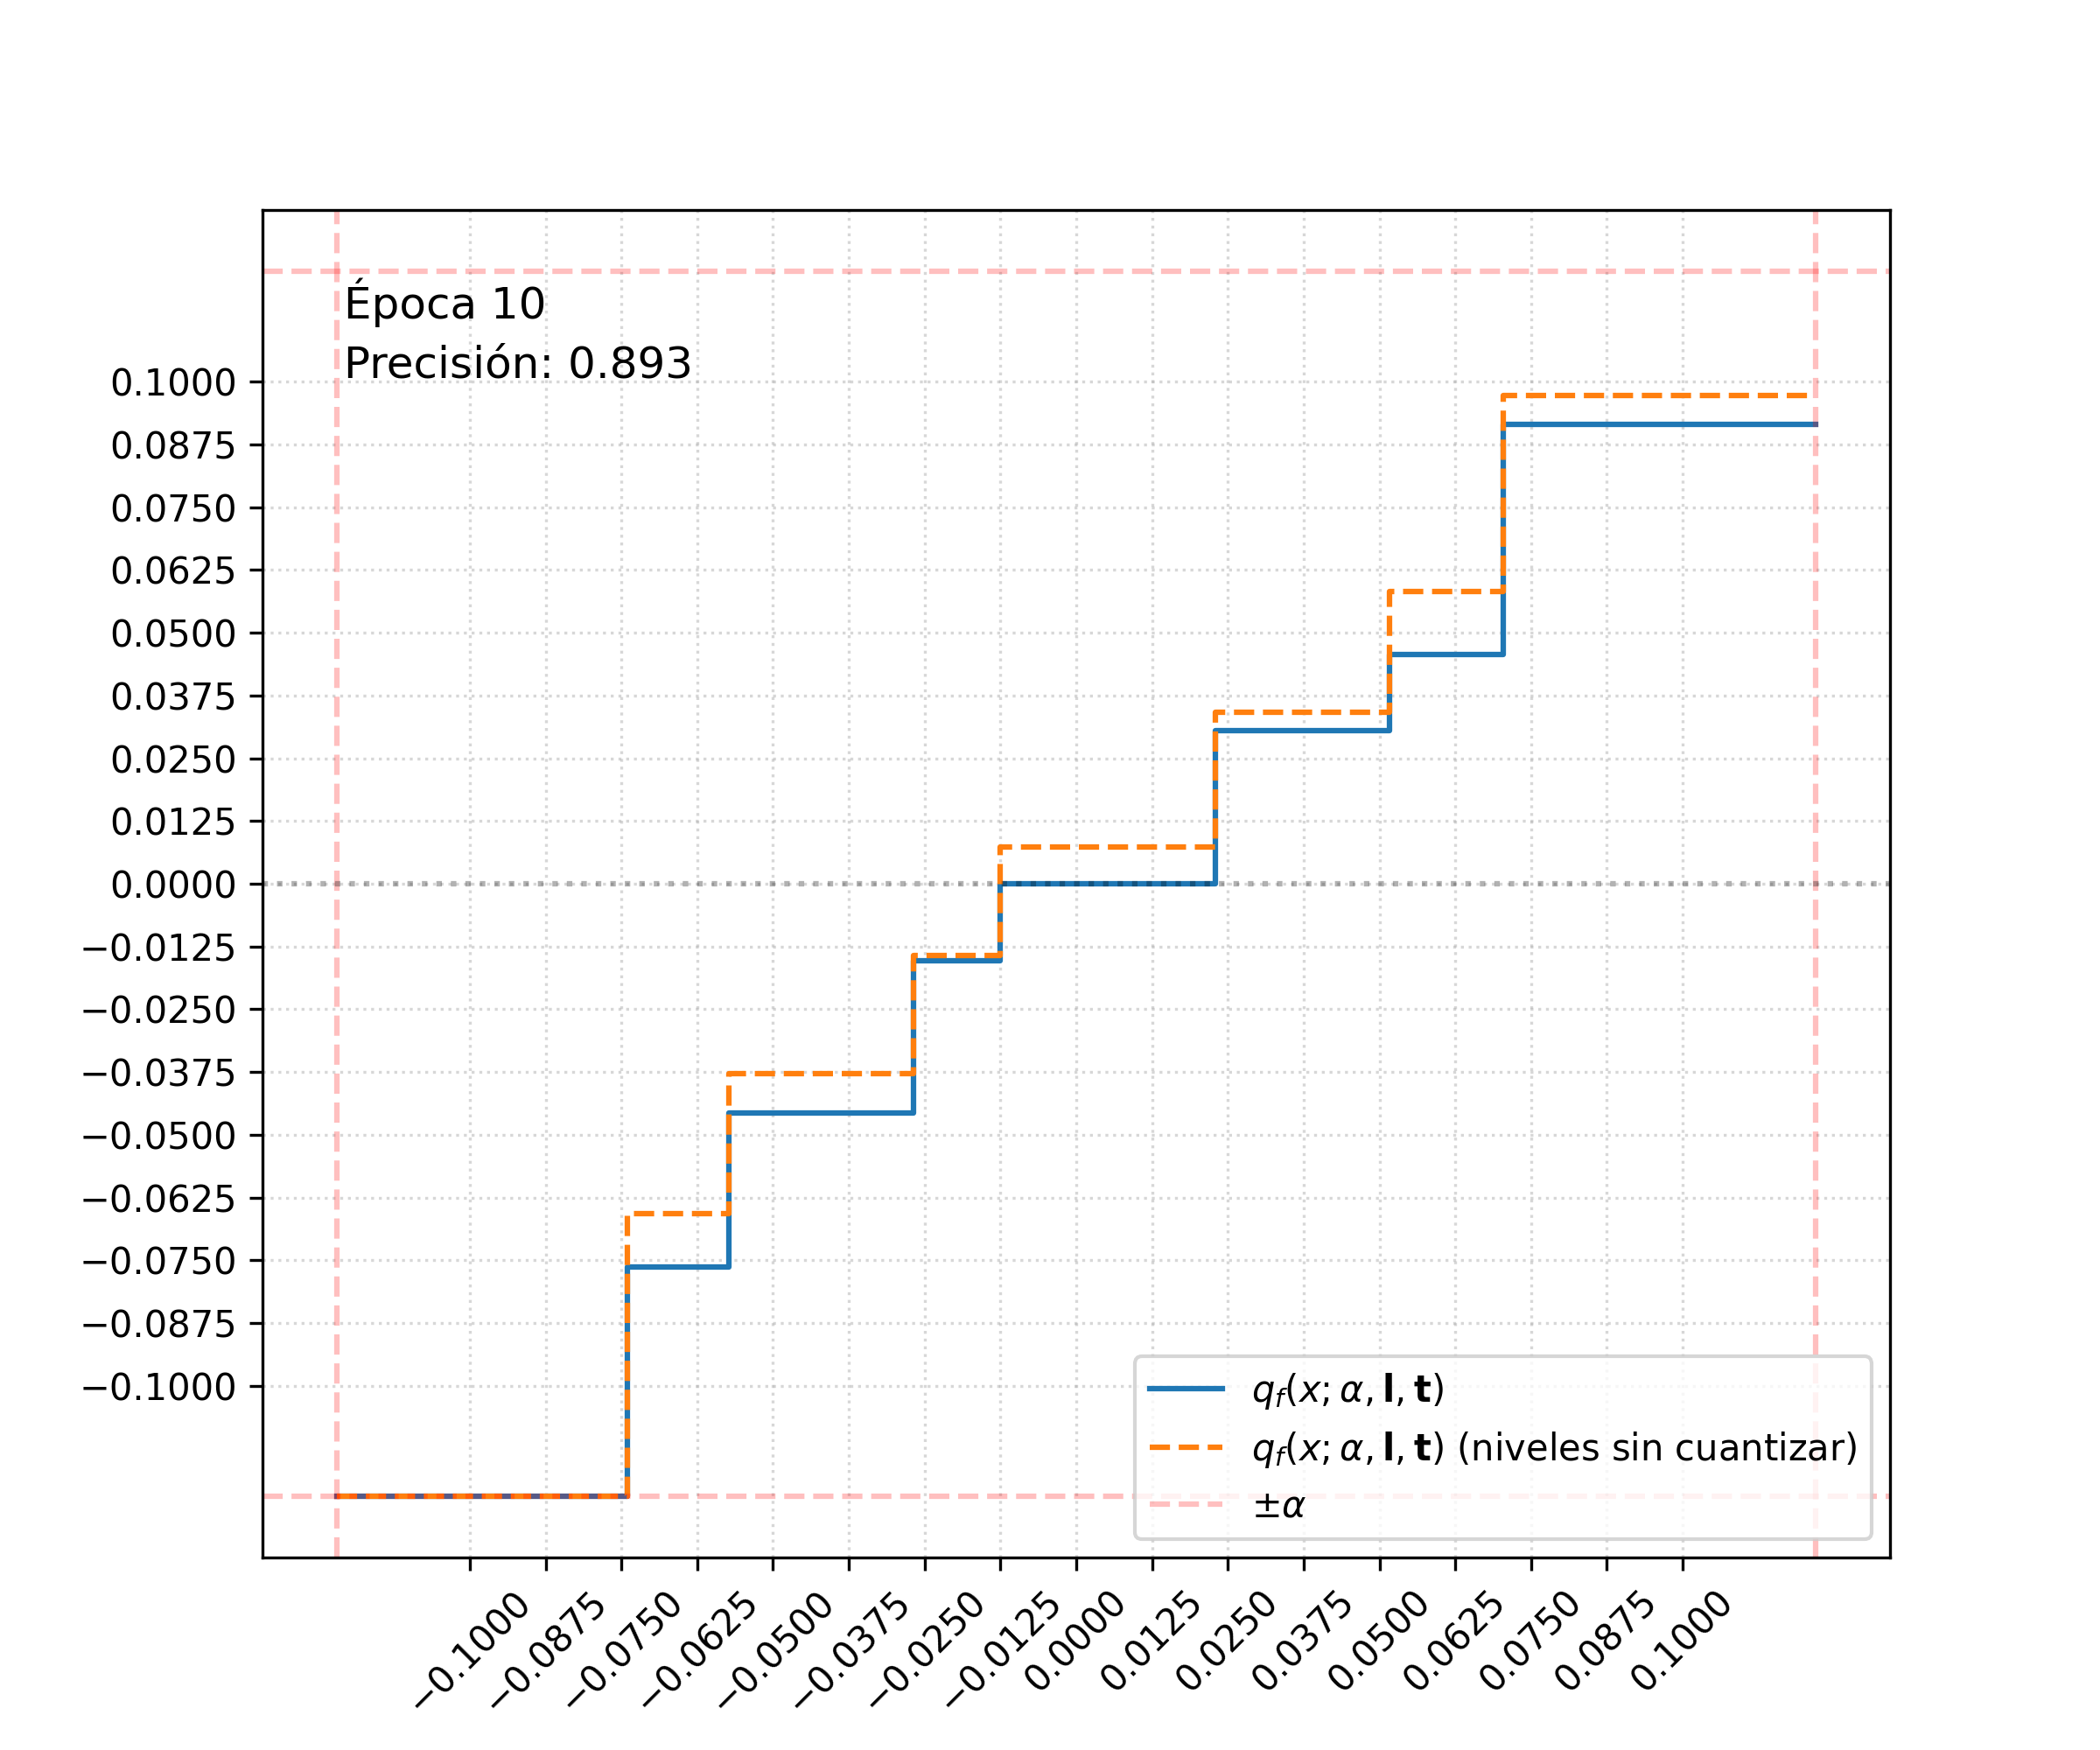
\includegraphics[width=\textwidth]{pics/quantizers/flex_ok/snapshot_00010.png}
        \caption{Época 10}
        \label{fig:flexible_snapshot_10}
    \end{subfigure}

    \caption{Evolución de la función de cuantización flexible durante el entrenamiento.}
    \label{fig:flexible_quantizer_snapshots}
\end{figure}
